\documentclass[11pt, a4paper]{article}
\usepackage[utf8]{inputenc}
\usepackage{circuitikz}
\usepackage{siunitx}
\usepackage{amsmath}
\usepackage[italian]{babel}
\usepackage{tablefootnote}
\usepackage{graphicx}
\usepackage{subcaption}
\usepackage{hyperref}

% Table padding
%\renewcommand{\arraystretch}{2}

\ctikzset{
    voltage/bump b=20pt,
    voltage/distance from node=0.5,
    voltage/european label distance=20pt,
}
%\everymath{\displaystyle}
\begin{document}

\title{Teoria dei Sistemi\\attività integrativa}
\author{Pietro De Nicolao}
\date{26 novembre 2015}
\maketitle
\tableofcontents
\newpage

\section*{Dati}
\begin{itemize}
    \item $\alpha = 0.04$
    \item $\beta = 0.18$
    \item $n = 16 \qquad [n]_3 = 1$
    \item $c = 4 \qquad [c]_3 = 1$
    \item $L = 12\,\textrm{nH}$
    \item $C = 12\,\textrm{pF}$
    \item $i = - \alpha x_2 + \beta x_2^3$
\end{itemize}


% -------- PUNTO 1 --------
\section{Equazioni di stato}
Considero l'equazione caratteristica del condensatore $C$:
\begin{equation}
\label{cond-caratt}
i_c = C \dot{x_2}
\end{equation}

Applico LKC al nodo A:
\begin{equation}
i_c = -x_1 - i
\end{equation}

Sostituendo $i_c$ nell'equazione~\ref{cond-caratt}, ottengo la prima equazione di stato:
\begin{equation}
\dot{x_2} = -\frac{1}{C} x_1 + \frac{1}{C}\left( \alpha x_2 - \beta x_2^3\right)
\end{equation}

Poi, considero l'equazione caratteristica del condensatore $L$:
\begin{equation}
\label{ind-caratt}
v_L = L \dot{x_1}
\end{equation}

Applico LKT alla maglia di sinistra, ottenendo:
\begin{equation}
x_2 = v_R + v_L = x_1 R + L \dot{x_1}
\end{equation}

Da cui la seconda equazione di stato:
\begin{equation}
    \dot{x_1} = -\frac{R}{L}x_1 + \frac{1}{L} x_2
\end{equation}

Il sistema è dunque descritto dalle equazioni:
\begin{equation}
    \left\{
    \begin{aligned}
        \dot{x_1} =& -\frac{\strut R}{\strut L}x_1 + \frac{1}{L} x_2\\
        \dot{x_2} =& -\frac{\strut 1}{\strut C} x_1 + \frac{1}{C}\left( \alpha x_2 - \beta x_2^3\right)\\
    \end{aligned}
    \right.
\end{equation}


% -------- PUNTO 2 --------
\section{Assenza di cicli per $R$ elevato}
L'assenza di cicli per particolari valori di $R$ può essere mostrata grazie al criterio di Bendixon.
\begin{equation}
    \textrm{div f}(x_1, x_2) = \frac{\partial f_1(x_1,x_2)}{\partial x_1} + \frac{\partial f_2(x_1,x_2)}{\partial x_2} = -\frac{R}{L} + \frac{\alpha}{C} - \frac{3\beta}{C}x_2^2
\end{equation}
\begin{equation}\label{big-resistance}
    R > \alpha \frac{L}{C} \Longrightarrow \textrm{div f}<0 \quad \forall x_2
\end{equation}
Per $R > \alpha \frac{L}{C} = 40 \Omega$, la divergenza assume valore negativo per qualunque $x_2$: dunque, non sono presenti cicli nell'intero piano.

Il risultato è in accordo con l'analogia intuitiva che associa la resistenza elettrica con l'attrito nei sistemi meccanici: entrambi i fenomeni dissipano energia e smorzano i movimenti periodici.


% -------- PUNTO 3 --------
\section{Equilibri}
Annullando le derivate delle equazioni del sistema, con semplici passaggi si ricavano le seguenti equazioni:

\begin{equation}
\left\{
\begin{aligned}
    &x_1 ( \beta R^3 x_1^2 - \alpha R + 1) = 0\\
    &x_2 = R x_1\\
\end{aligned}
\right.
\end{equation}

Dunque esiste sempre l'equilibrio banale $x_1 = x_2 = 0$.
Se $R \le \frac{1}{\alpha}$, allora il termine $( \beta R^3 x_1^2 - \alpha R + 1)$ è sempre positivo o nullo e non vi sono altri equilibri.

Altrimenti, esistono altri due equilibri oltre a quello banale.

\begin{table}
    \centering
    \begin{tabular}{l | l}
        \textbf{R} & \textbf{Equilibri}\\
        \hline
        $R \le \dfrac{\strut 1}{\strut\alpha}$ & $(0, 0)$\\
        $R > \dfrac{\strut 1}{\strut\alpha}$ & $(0,0),
        \left( \pm \sqrt{\dfrac{\strut\alpha R -1}{\strut\beta R^3}}, \pm \sqrt{\dfrac{\alpha R -1}{\beta R}} \right)$
    \end{tabular}
    \caption{Equilibri del sistema al variare di $R$.}
\end{table}

\subsection{Stabilità}
Lo jacobiano del sistema linearizzato è:
\begin{equation}
J(x_1,x_2) =
\begin{bmatrix}
-\dfrac{\strut R}{L\strut} & \dfrac{1}{L} \\
-\dfrac{\strut 1}{C\strut} & \dfrac{\alpha}{C}-\dfrac{\beta}{C} 3x_2^2 \\
\end{bmatrix}
\end{equation}

Analizziamo ora il tipo degli equilibri.
\begin{enumerate}
\item (0,0)\\
\begin{equation}
    J(0,0) =
    \begin{bmatrix}
    -\dfrac{\strut R}{L\strut} & \dfrac{1}{L} \\
    -\dfrac{\strut 1}{C\strut} & \dfrac{\alpha}{C} \\
    \end{bmatrix}
\end{equation}

\begin{equation}
\textrm{tr } J(0,0) = \frac{L\alpha-CR}{CL}
\end{equation}
\begin{equation}
\det J(0,0) = \frac{1-r\alpha}{CL}
\end{equation}
L'analisi di stabilità dell'equilibrio è mostrata nella tabella~\ref{stab-00}.

\begin{table}
    \centering
    \begin{tabular}{l l l l l}
        & & tr $J(0,0)$ & $\det J(0,0)$ & tipo\\
        \hline
        $R<\dfrac{1\strut}{\alpha\strut}$ & $(0, 25 \Omega)$ & $>0$ & $>0$ & instabile \\
        \hline
        $\dfrac{1\strut}{\alpha\strut}<R<\dfrac{L\alpha}{C}$ & $(25 \Omega, 40 \Omega)$ & $>0$ & $<0$ & sella \\
        \hline
        $R>\dfrac{L\alpha\strut}{C\strut}$ & $(40 \Omega, +\infty)$ & $<0$ & $<0$ & sella \\
        \hline
    \end{tabular}
    \caption{Stabilità dell'equilibrio $(0,0)$ al variare di R.}
    \label{stab-00}
\end{table}

\item $\left( \pm \sqrt{\dfrac{\strut\alpha R -1}{\strut\beta R^3}}, \pm \sqrt{\dfrac{\alpha R -1}{\beta R}} \right)$

Questi equilibri esistono solo per $R > \frac{1}{\alpha}$, condizione che dunque può essere assunta nello studio della loro stabilità.

\begin{equation}
    J\left( \pm \sqrt{\dfrac{\strut\alpha R -1}{\strut\beta R^3}}, \pm \sqrt{\dfrac{\alpha R -1}{\beta R}} \right) =
    \begin{bmatrix}
        -\dfrac{R\strut}{L\strut} & \dfrac{1}{L} \\
        -\dfrac{1\strut}{C\strut} & \dfrac{3-2R\alpha}{CR} \\
    \end{bmatrix}
\end{equation}

\begin{equation}
    \det J = 2 \dfrac{R\alpha-1}{CL} > 0 \quad \forall R > \frac{1}{\alpha}
\end{equation}

\begin{equation}
    \textrm{tr } J = \dfrac{-CR^2+3L-2RL\alpha}{CRL}
\end{equation}

\begin{table}
    \centering
    \begin{tabular}{l l l l l}
        & & tr $J$ & $\det J$ & tipo\\
        \hline
        $\dfrac{1\strut}{\alpha\strut}<R<k$\tablefootnote{$k=\dfrac{-L\alpha + \sqrt{L^2\alpha^2+3LC}}{C} = 27.82 \Omega$}
        & $(25 \Omega, 27.82 \Omega)$ & $>0$ & $>0$ & fuoco instabile \\
        \hline
        $R>k$ & $(27.82 \Omega, +\infty)$ & $<0$ & $>0$ & fuoco stabile \\
        \hline
    \end{tabular}
    \caption{Stabilità dell'equilibrio $\left( \pm \sqrt{\frac{\alpha R -1}{\beta R^3}}, \pm \sqrt{\frac{\alpha R -1}{\beta R}} \right)$ al variare di R.}
    \label{stab-eq2}
\end{table}

\subsection{Biforcazioni degli stati di equilibrio}
Le biforcazioni del sistema al variare di $R$ sono elencate in~\autoref{tab:biforc-r}.
Il sistema ammette una biforcazione forcone, due Hopf, una doppia omoclina e una biforcazione tangente di cicli. I valori di $R$ a cui si presentano le biforcazioni doppia omoclina e tangente di cicli sono stati ricavati empiricamente simulando il sistema con Pplane.

\begin{table}
    \centering
    \begin{tabular}{l l p{0.5\linewidth}}
        $\mathbf{R}$ & \textbf{Tipo} & \textbf{Note}\\
        \hline
        $\frac{1}{\alpha} = 25 \Omega$ & forcone & per $R>25 \Omega$ nascono due equilibri instabili (\autoref{fig:forcone}) \\
        \hline
        $k=27.82 \Omega$ & Hopf (doppia) & intorno ai due rami del forcone si creano cicli instabili; i due equilibri diventano stabili (\autoref{fig:hopf}) \\
        \hline
        $28.35 \Omega$ & doppia omoclina & i cicli generati dalle Hopf collidono con la sella in $(0,0)$; si crea un nuovo ciclo instabile interno (\autoref{fig:dopo-omoclina}) \\
        \hline
        $28.49 \Omega$ & tangente di cicli & il ciclo instabile interno e quello stabile esterno collidono e spariscono \\
        \hline
    \end{tabular}
    \caption{Biforcazioni del sistema al variare di $R$.}
    \label{tab:biforc-r}
\end{table}

\begin{figure}
    \centering
    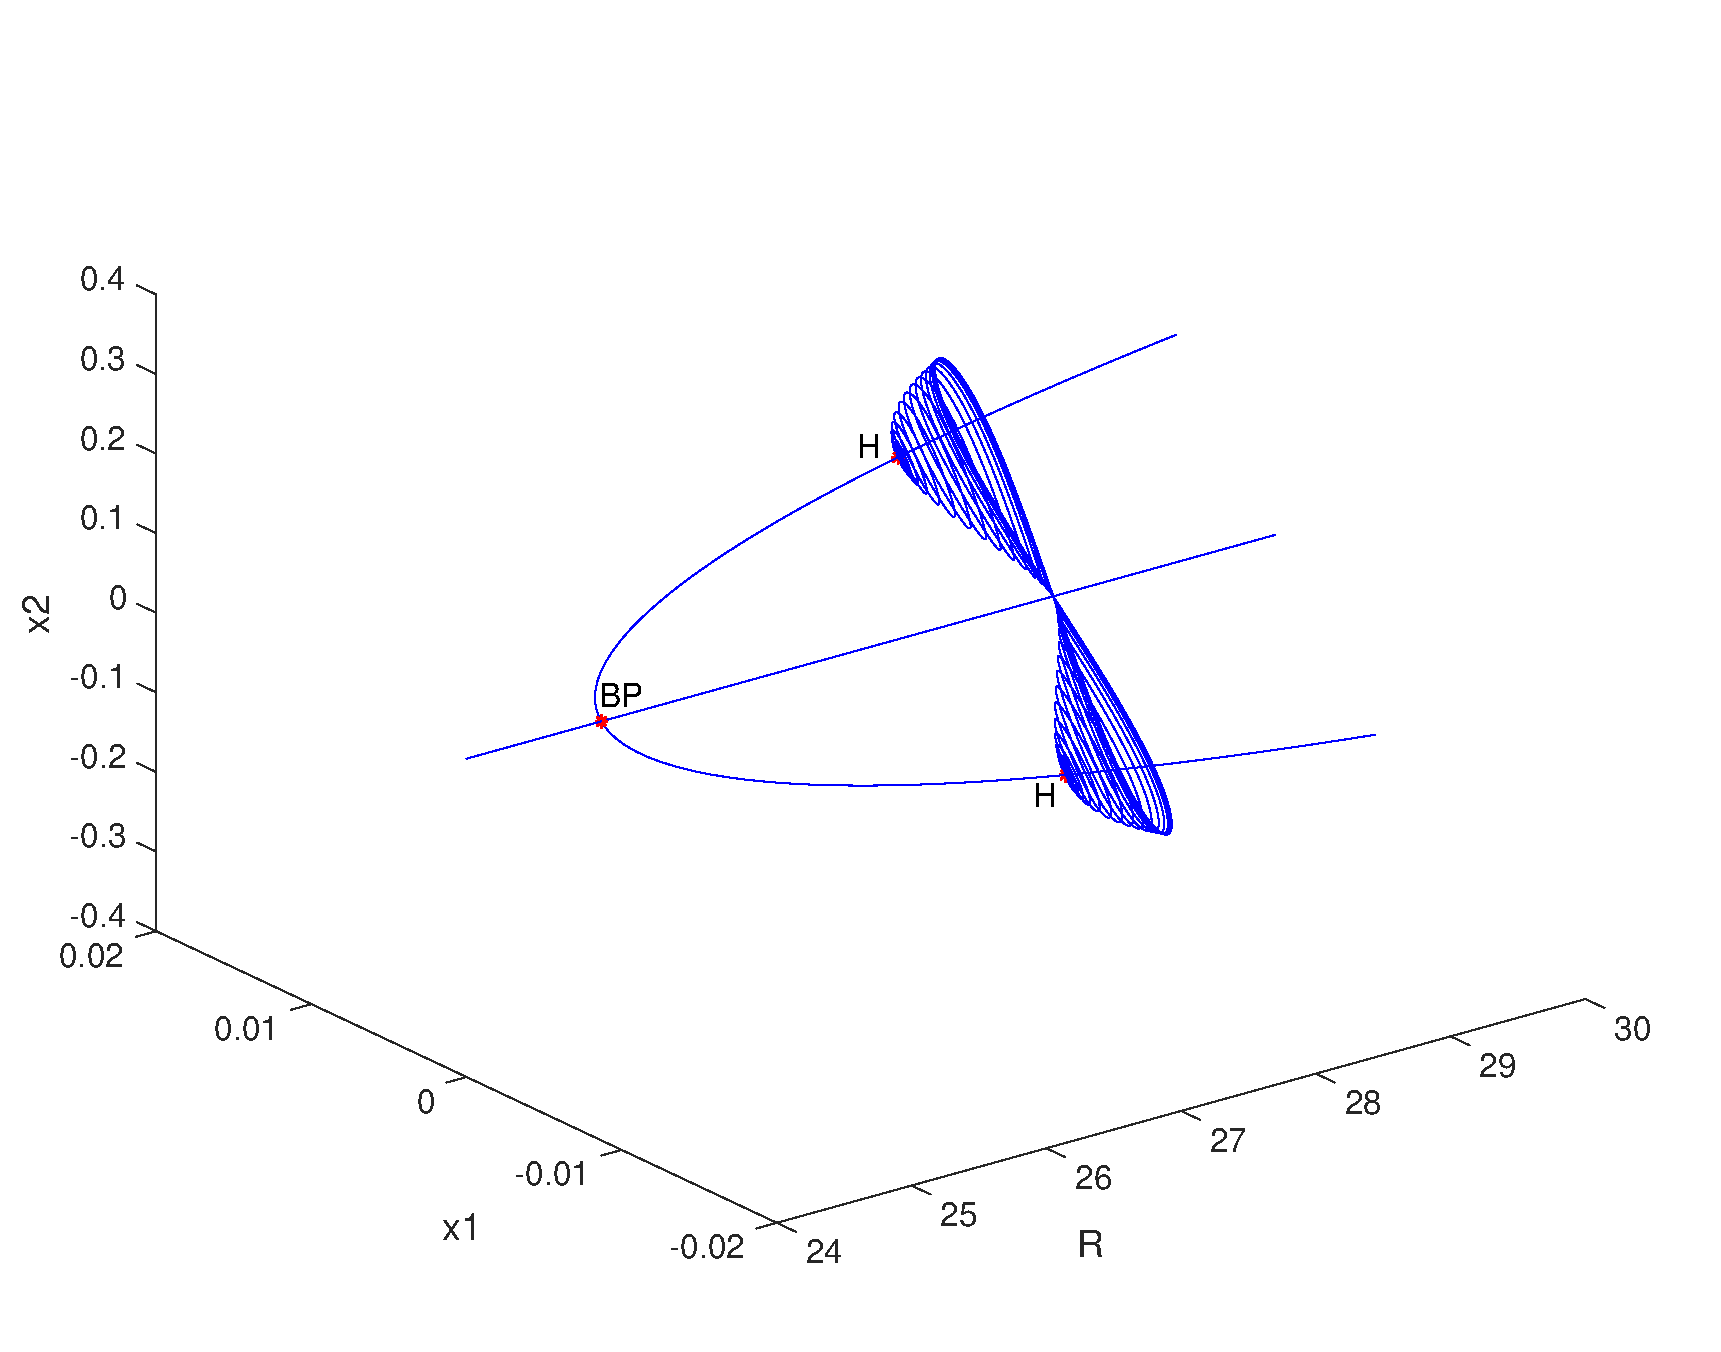
\includegraphics[width=1.1\textwidth]{matcont/ForconeHopf}
    \caption{Le biforcazioni forcone e Hopf.}
    \label{fig:forcone}
\end{figure}

\subsection{Cicli}
Per $R<\frac{1}{\alpha}=25 \Omega$, il sistema ammette un ciclo stabile che contiene l'equilibrio instabile.

Per $\frac{1}{\alpha} < R < k$, il sistema ammette un ciclo stabile che contiene l'origine (sella) e i due equilibri instabili, compatibilmente con il criterio di Poincaré.

\begin{figure}
\centering
    \begin{subfigure}[b]{0.8\textwidth}
            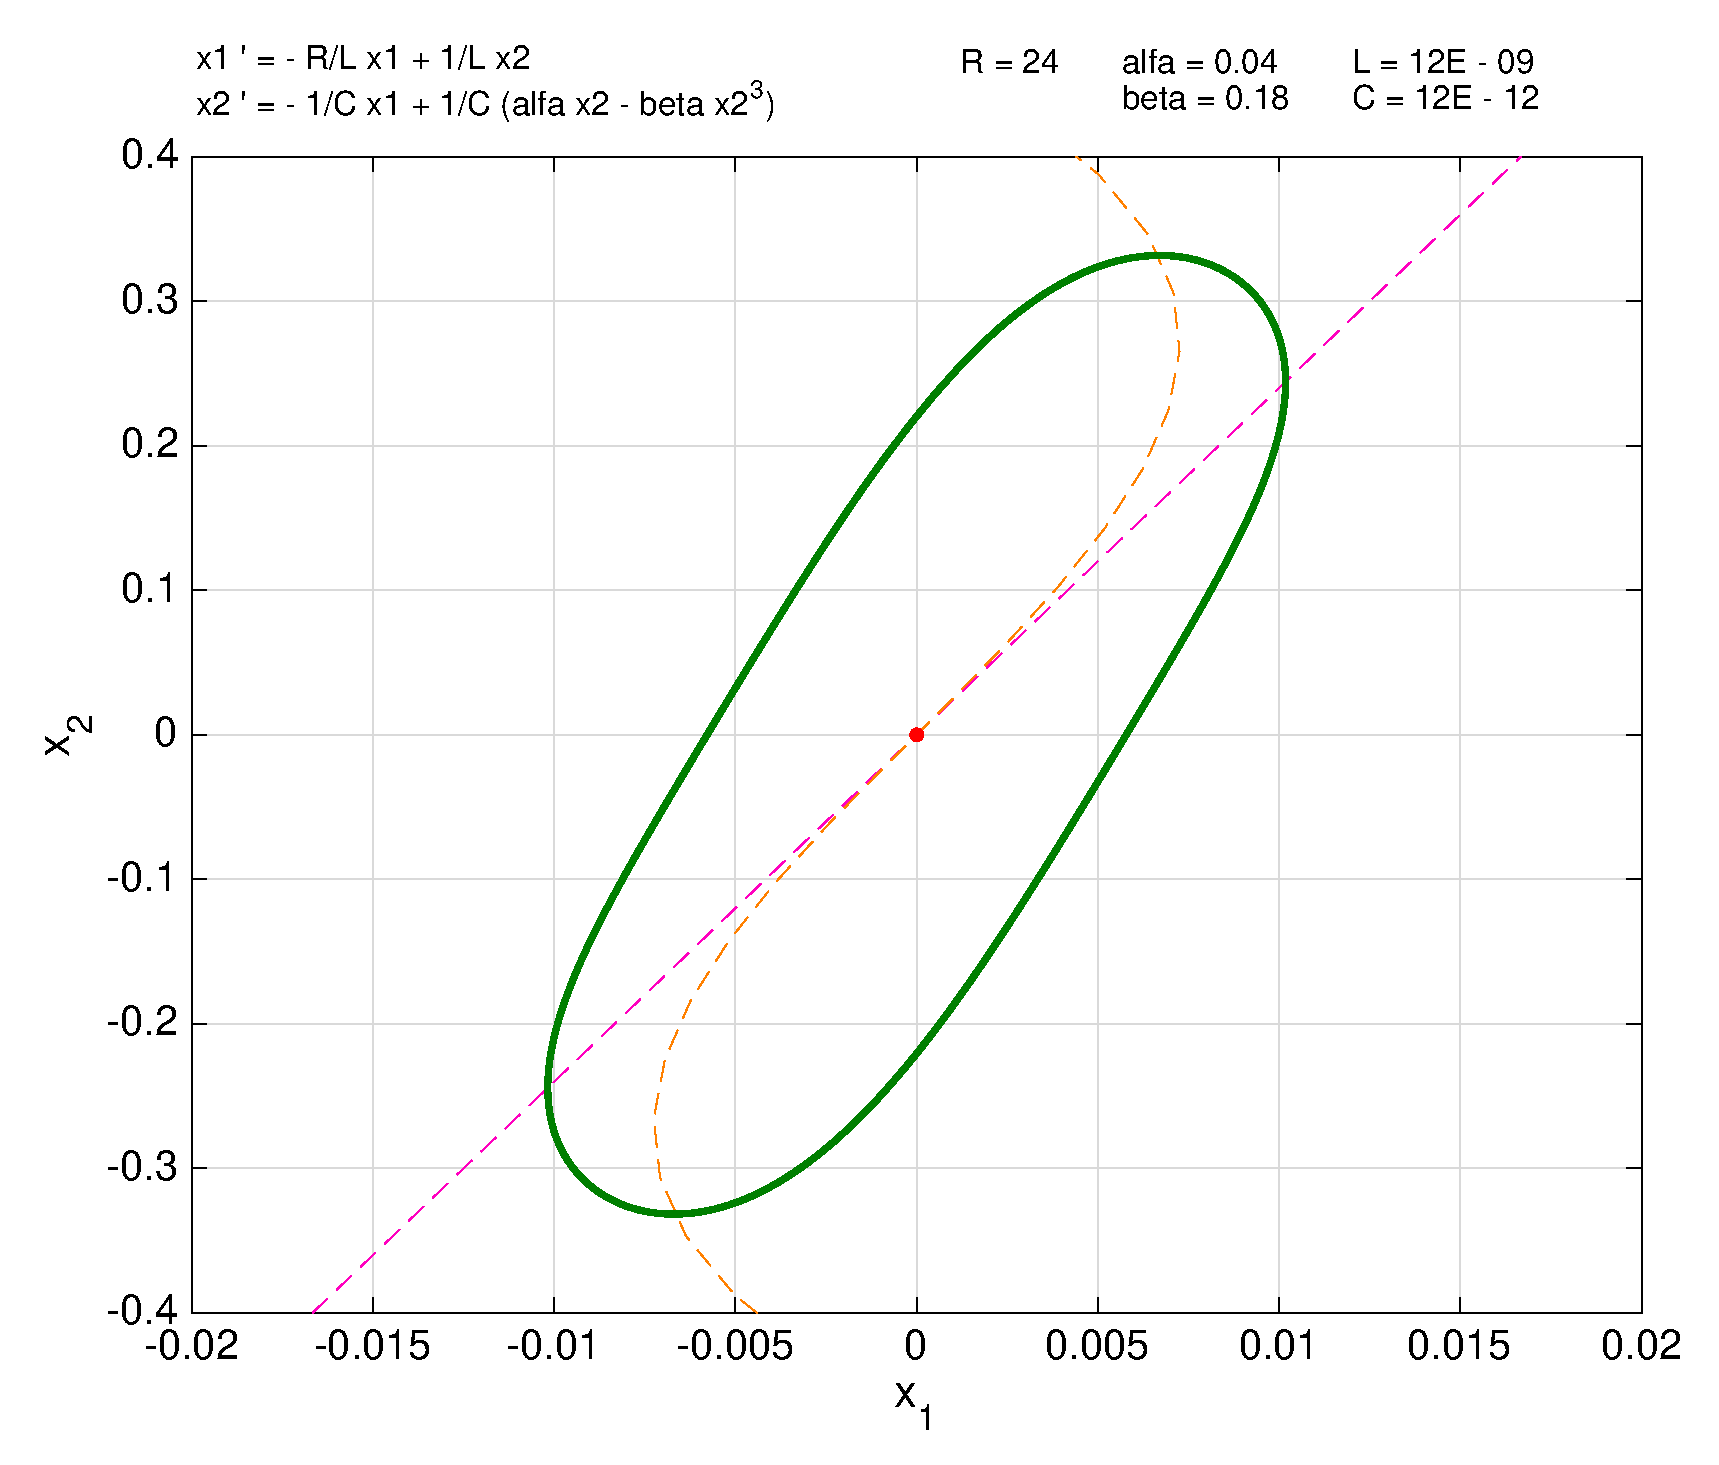
\includegraphics[width=\textwidth]{pplane/Cycle24ohm}
            \caption{Ciclo stabile per $R = 24 \Omega$.}
    \end{subfigure}
    \par\bigskip
    \begin{subfigure}[b]{0.8\textwidth}
            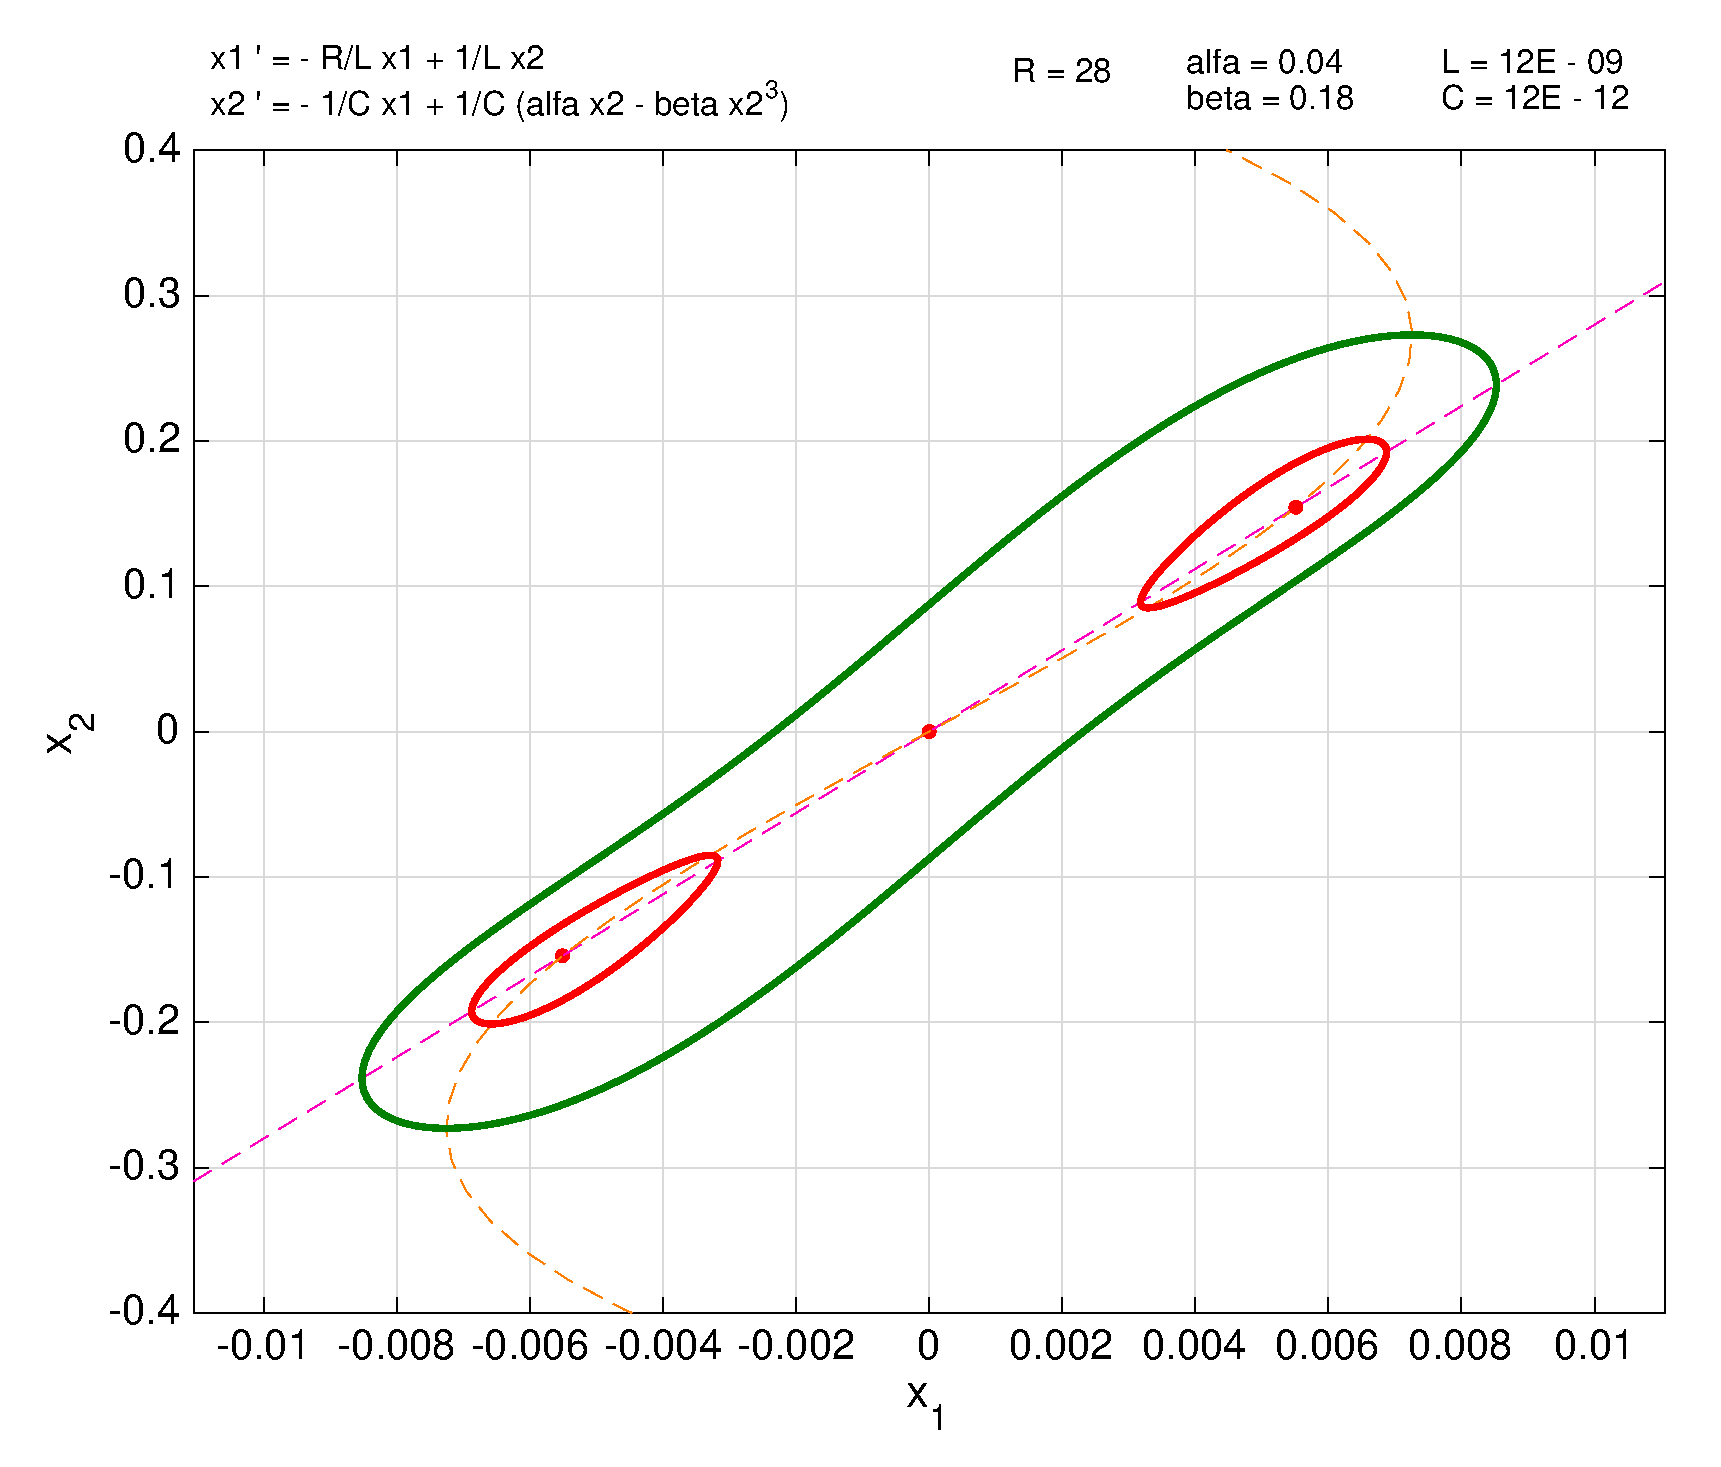
\includegraphics[width=\textwidth]{pplane/Cycle26ohm}
            \caption{Ciclo stabile (esterno) e cicli instabili (interni) per $R = 26 \Omega$.}
            \label{fig:hopf}
    \end{subfigure}
    \caption{Cicli prima e dopo la biforcazione di Hopf.}
    \label{fig:cicli-hopf}
\end{figure}

\begin{figure}
    \centering
    \begin{subfigure}[b]{0.8\textwidth}
            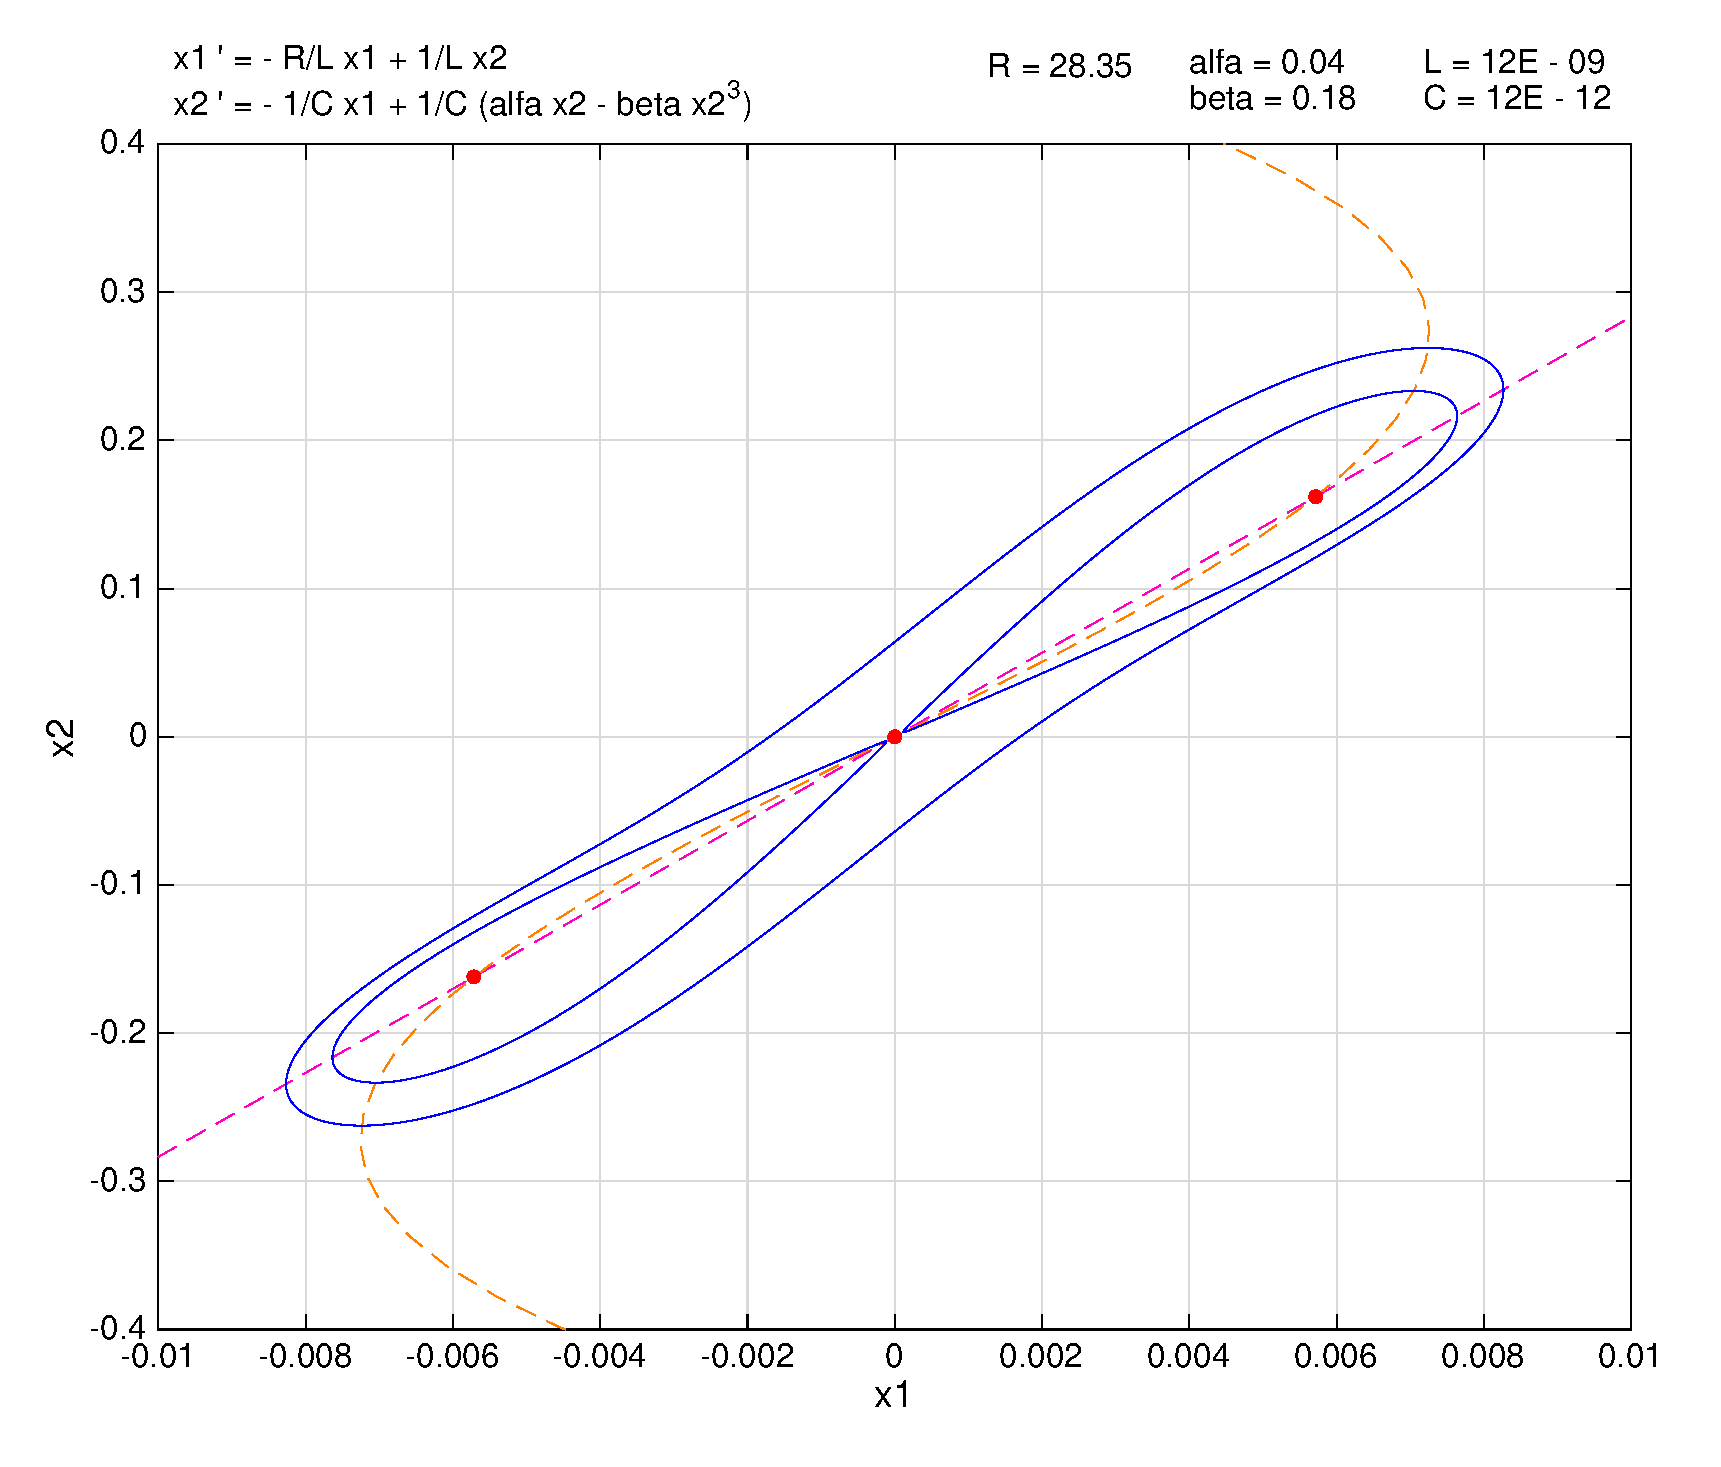
\includegraphics[width=\textwidth]{pplane/DoppiaOmoclina}
            \caption{I due cicli instabili toccano la sella in $(0,0)$ subito prima della biforcazione omoclina.}
    \end{subfigure}
    \par\bigskip
    \begin{subfigure}[b]{0.8\textwidth}
            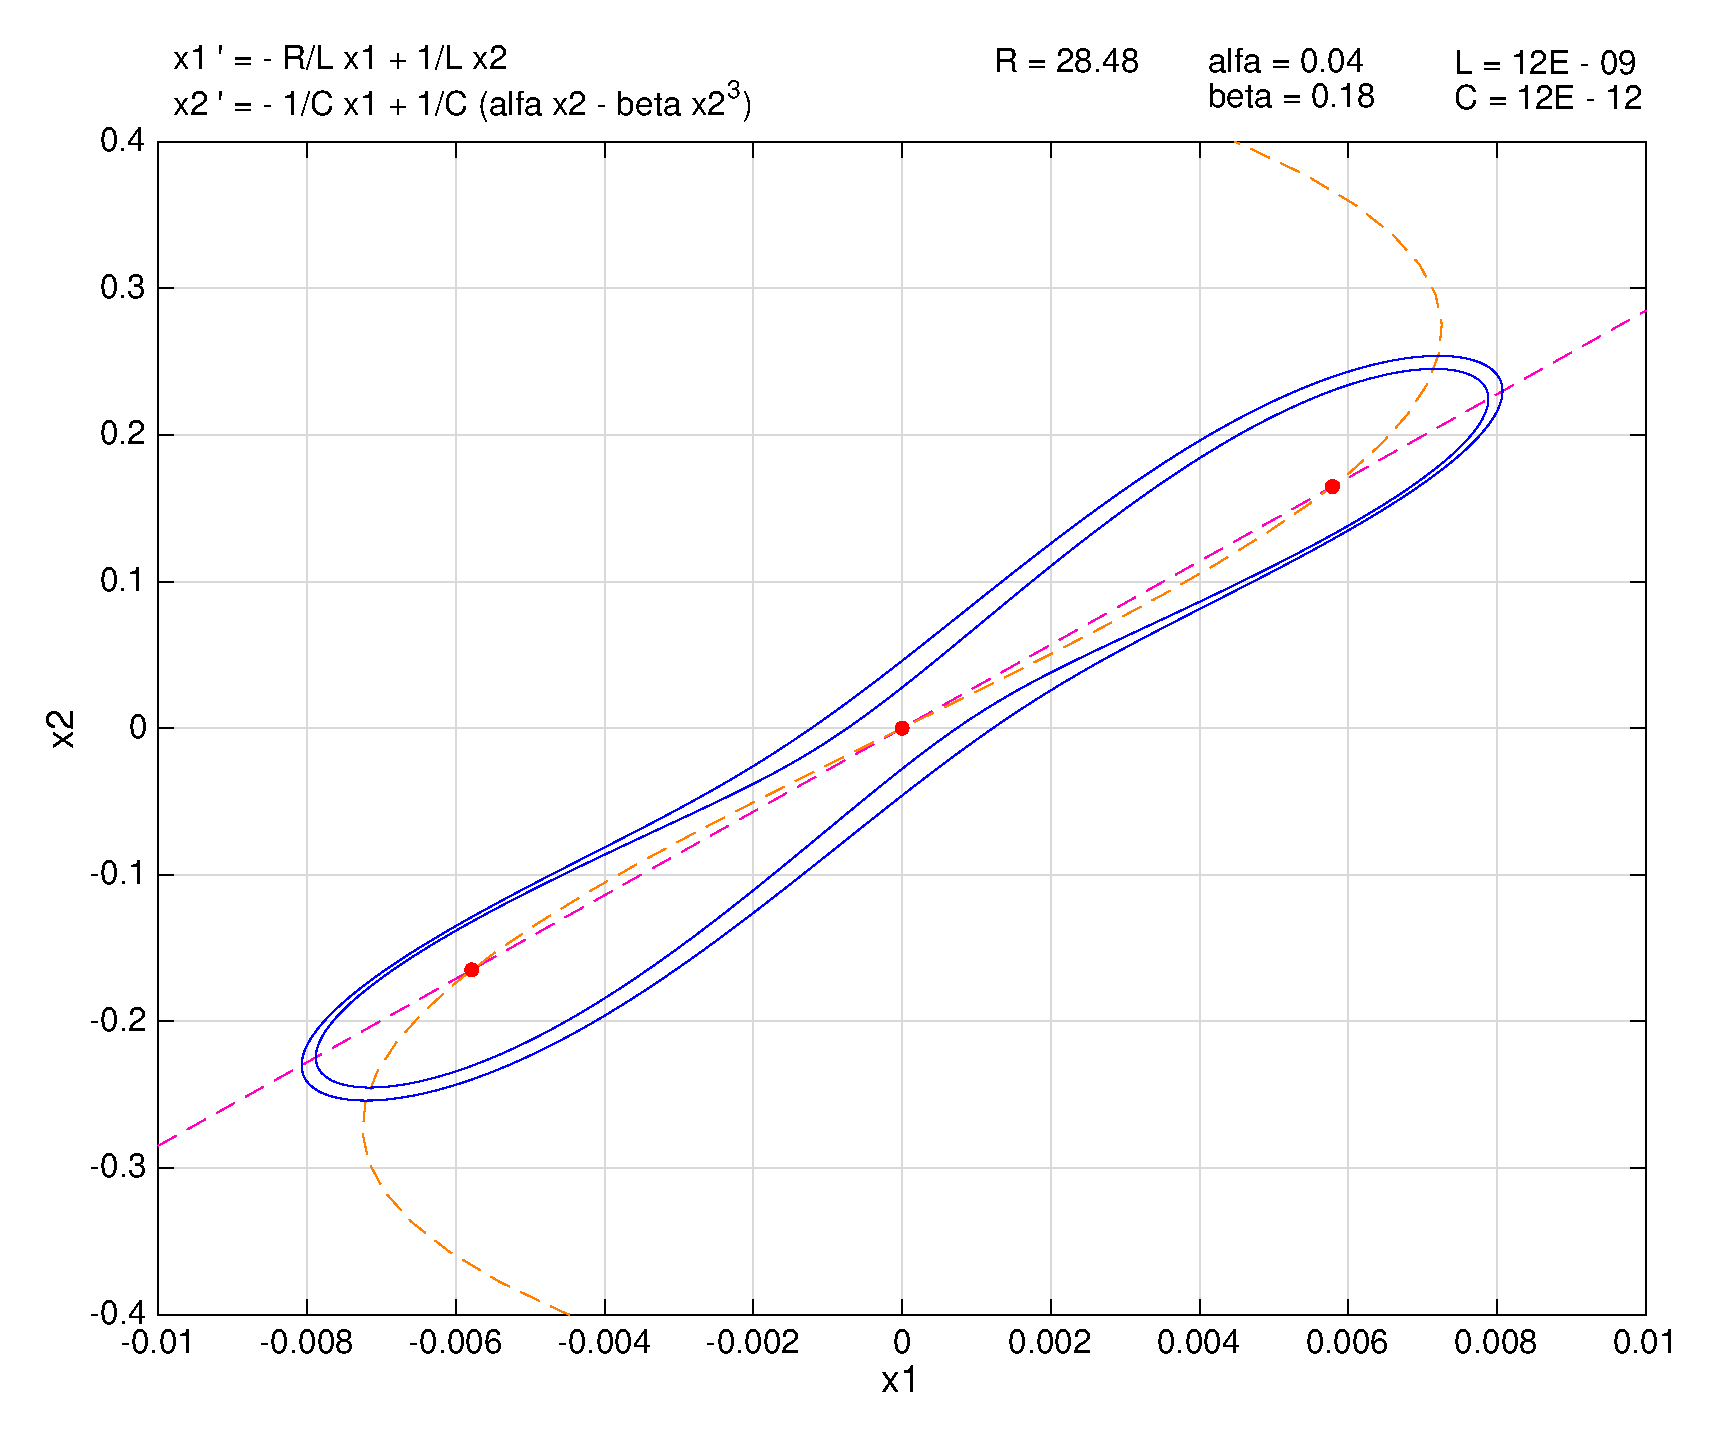
\includegraphics[width=\textwidth]{pplane/TangenteCicli}
            \caption{Dopo la biforcazione omoclina i due cicli instabili si sono fusi; qui sono mostrati immediatamente prima della tangente di cicli.}
            \label{fig:dopo-omoclina}
    \end{subfigure}
    \caption{Cicli prima e dopo la biforcazione omoclina.}
    \label{fig:cicli-omoclina}
\end{figure}


% -------- PUNTO 4 --------
\section{Diagramma delle biforcazioni}

Il diagramma delle biforcazioni è riportato in~\autoref{fig:biforcazioni-completo}.

\begin{figure}[h]
\centering
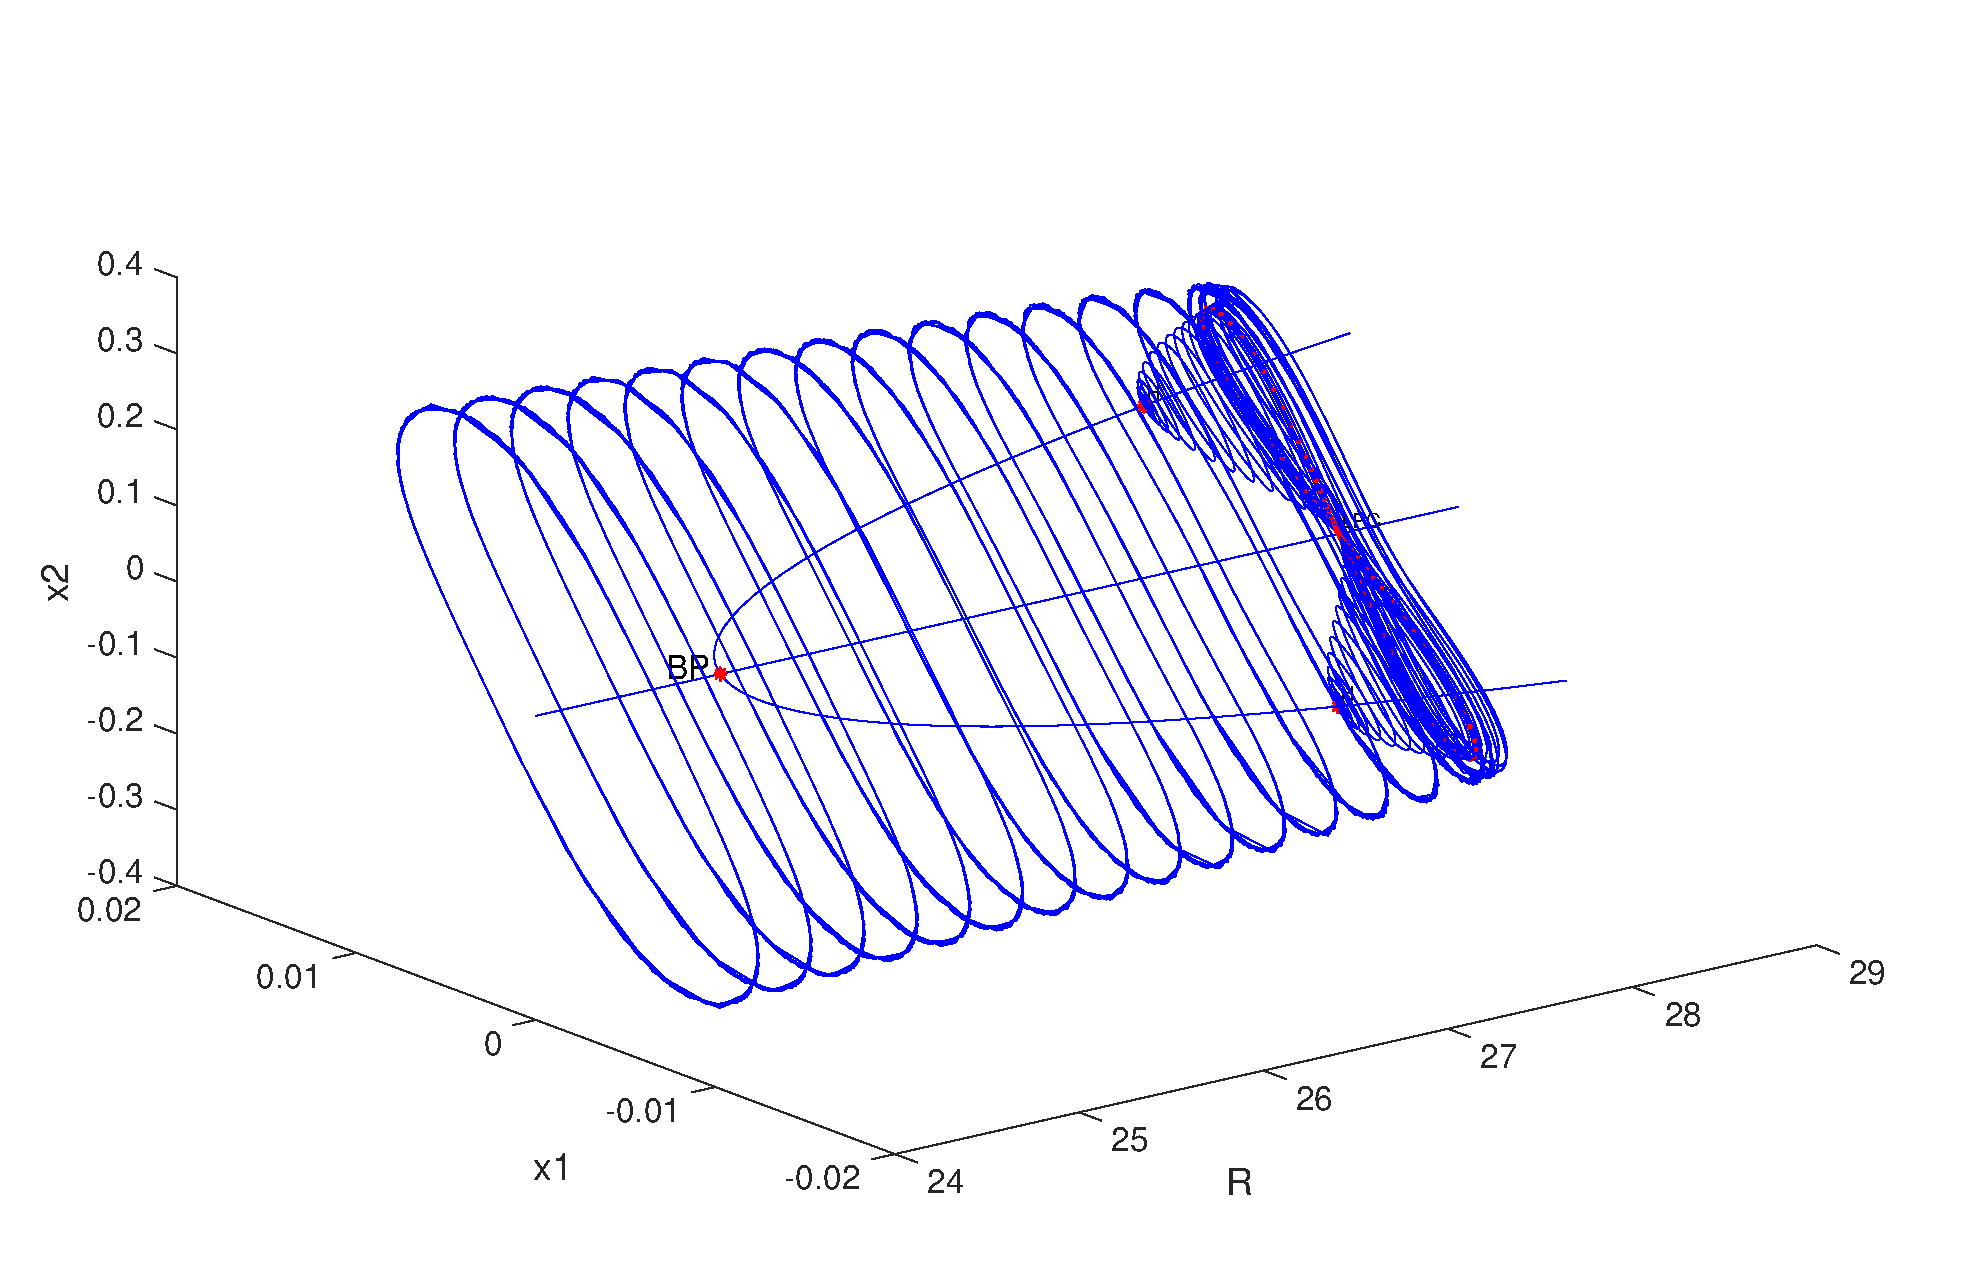
\includegraphics[width=0.8\textwidth]{matcont/BiforcazioniCompleto}
\caption{Il diagramma completo delle biforcazioni in funzione di $R$.}
\label{fig:biforcazioni-completo}
\end{figure}


% -------- PUNTO 5 --------
\section{Numero di biforcazioni trovate}
Il numero di biforcazioni trovate è riportato in~\autoref{tab:num-bif}.
\begin{table}[h]
    \centering
\begin{tabular}{| l | l |}
\hline
forcone & 1 \\
\hline
Hopf & 2 \\
\hline
doppia omoclina & 1 \\
\hline
tangente di cicli & 1 \\
\hline
\end{tabular}
\caption{Numero di biforcazioni del sistema.}
\label{tab:num-bif}
\end{table}


% -------- PUNTO 6 --------
\section{Comportamento caotico del sistema}

Si suppone che la resistenza $R$ del sistema vari periodicamente del 25\% seguendo la legge:
\begin{equation}
    R(t) = \bar{R} (1+0.25 \sin(\omega t))
    \label{eq:resistenza-var}
\end{equation}

Per mantenere il sistema autonomo e poterlo quindi simulare, si possono introdurre due nuove equazioni relative a due nuove variabili di stato, disaccoppiate dalle precedenti.
Il sistema diventa dunque:

\begin{equation}
    \left\{
    \begin{aligned}
        R =& \bar{R} (1+0.25 x_4) \\
        \dot{x_1} =& -\frac{\strut R}{\strut L}x_1 + \frac{1}{L} x_2\\
        \dot{x_2} =& -\frac{\strut 1}{\strut C} x_1 + \frac{1}{C}\left( \alpha x_2 - \beta x_2^3\right)\\
        \dot{x_3} =& x_3 - \omega x_4 - (x_3^2+x_4^2) x_3 \\
        \dot{x_4} =& \omega x_3 + x_4 - (x_3^2+x_4^2) x_4 \\
    \end{aligned}
    \right.
    \label{eq:sistema-chaos}
\end{equation}

Dove è immediato verificare per sostituzione che
\begin{equation}
    \begin{aligned}
        x_3 =& \cos (\omega t)\\
        x_4 =& \sin (\omega t)\\
    \end{aligned}
\end{equation}

Dall'equazione~\ref{eq:resistenza-var} si osserva che, per valori di $\bar{R}$ ragionevoli ($29.5 \Omega$ ad esempio) l'oscillazione è sufficientemente ampia da passare per tutti i punti di biforcazione (\autoref{tab:biforc-r}): non è davvero necessario variare $\bar{R}$ per trovare il caos.

La precedente osservazione semplifica molto il problema, che si riduce a trovare un giusto valore del solo parametro $\omega$ per cui il sistema presenti comportamento caotico.

Provando a calcolare sistematicamente gli esponenti di Lyapunov del sistema~\ref{eq:sistema-chaos} per valori di $\omega$ nell'ordine di grandezza dell'unità, si ottiene il risultato illustrato in~\autoref{fig:lyapunov-plot}.

\begin{figure}
    \centering
    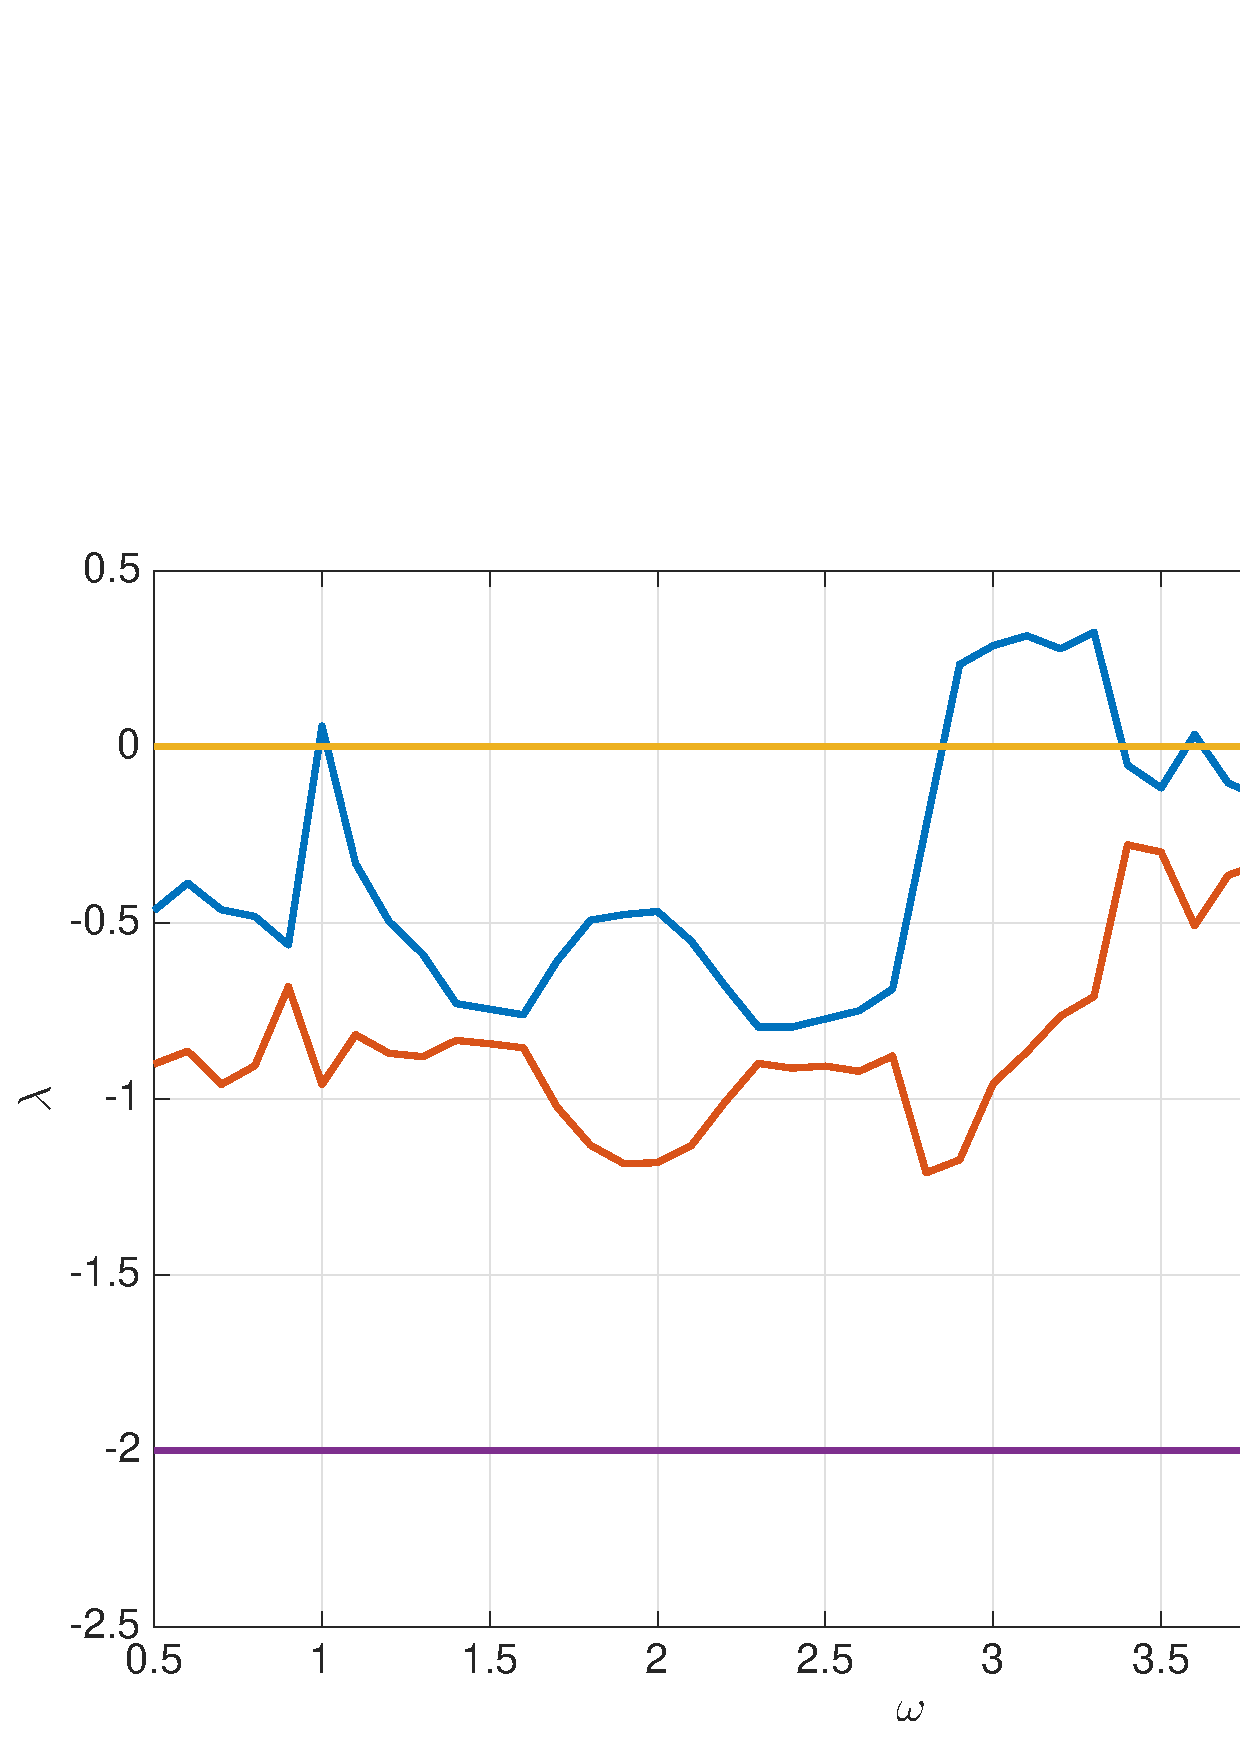
\includegraphics[width=\textwidth]{matcont/LyapunovPlot}
    \caption{Esponenti di Lyapunov del sistema~\ref{eq:sistema-chaos} calcolati per $\omega \in [0.5, 5]$, $\bar{R}=29.5 \Omega$.}
    \label{fig:lyapunov-plot}
\end{figure}

Integrando per intervalli estesi il sistema, si verifica che effettivamente per $\omega = 3.1415$ gli esponenti di Lyapunov valgono: $[0.28, 0, -0.77, -2]$.

Ciò dimostra il comportamento caotico del sistema. Lo strano attrattore simulato per gli stessi parametri è mostrato in~\autoref{fig:strano-attrattore}, insieme alla sua sezione di Poincaré in~\autoref{fig:chaos-poincare}.

\begin{figure}
    \centering
    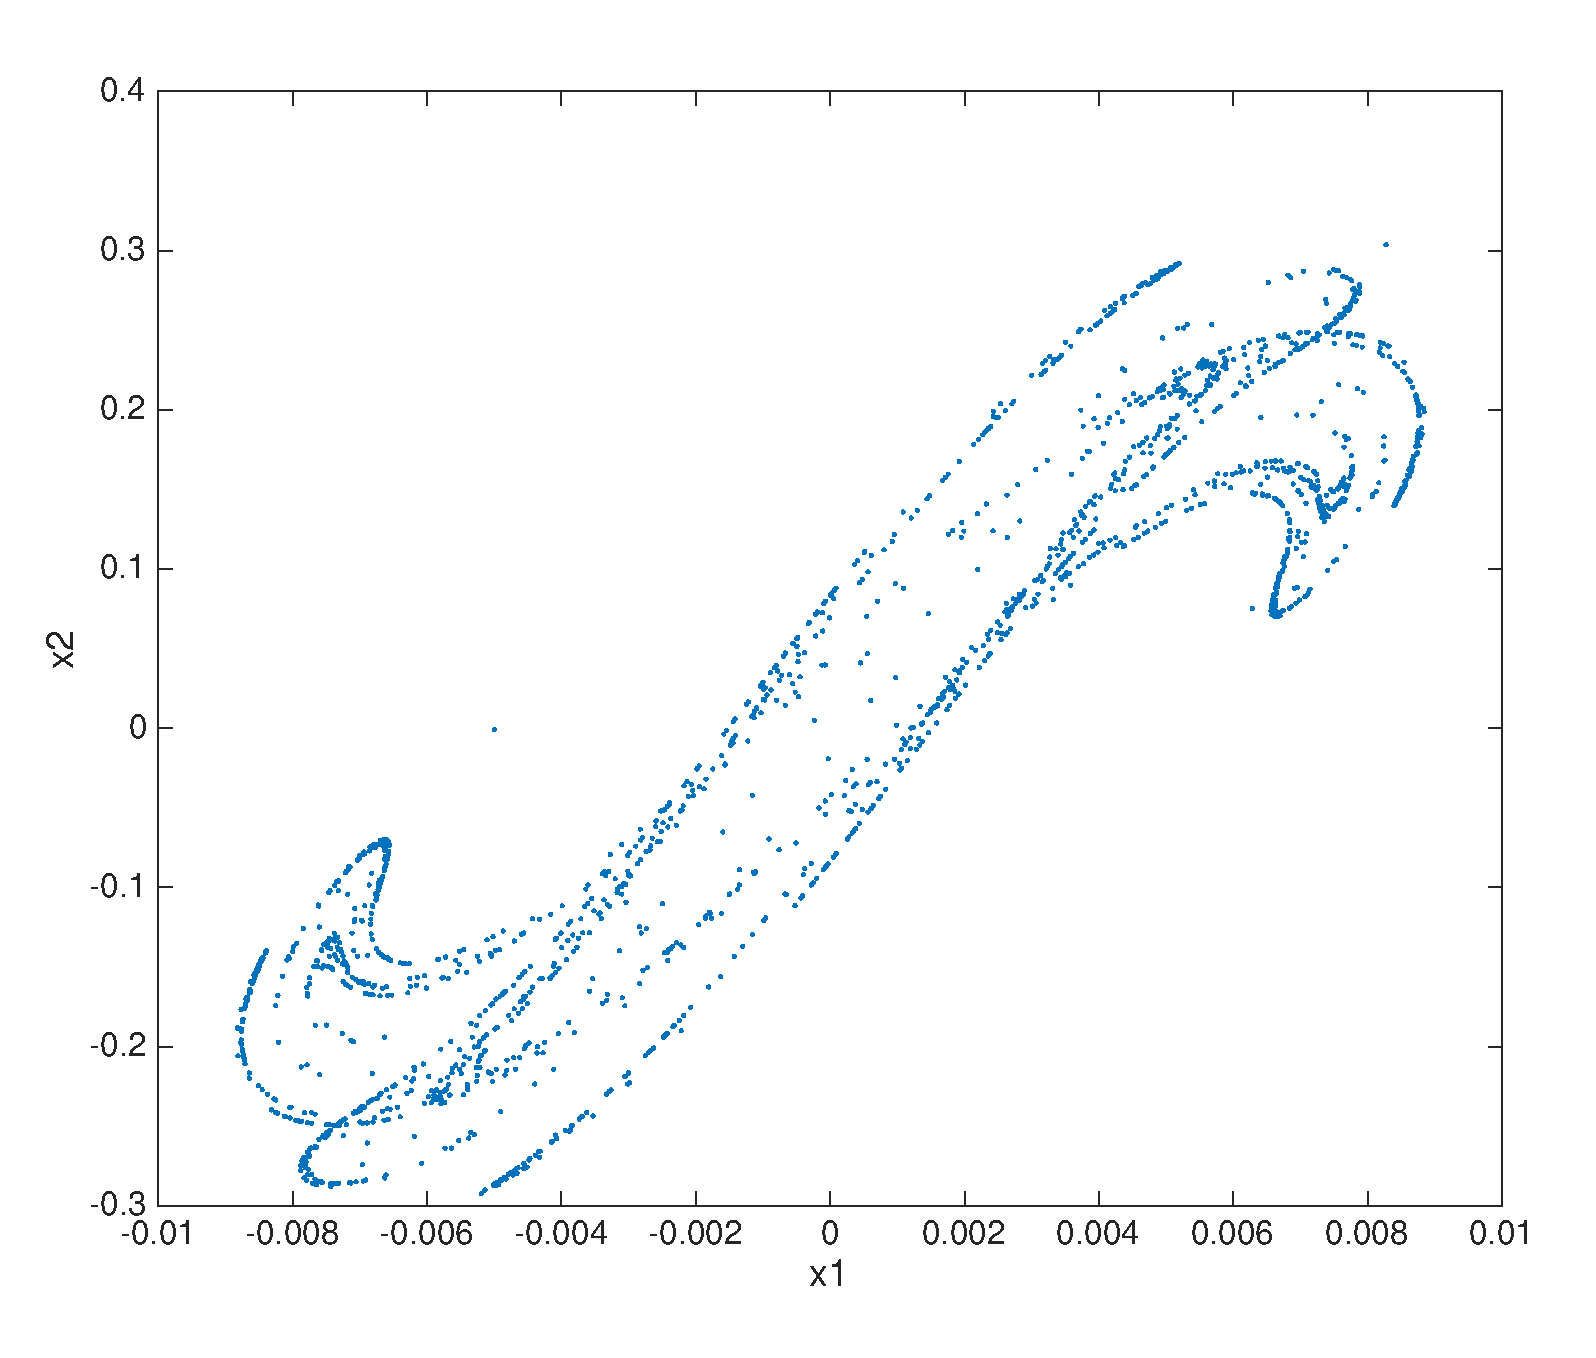
\includegraphics[width=\textwidth]{matcont/PoincareCaos}
    \caption{La mappa di Poincaré dello strano attrattore.}
    \label{fig:chaos-poincare}
\end{figure}

\begin{figure}
    \centering
    \begin{subfigure}{\textwidth}
        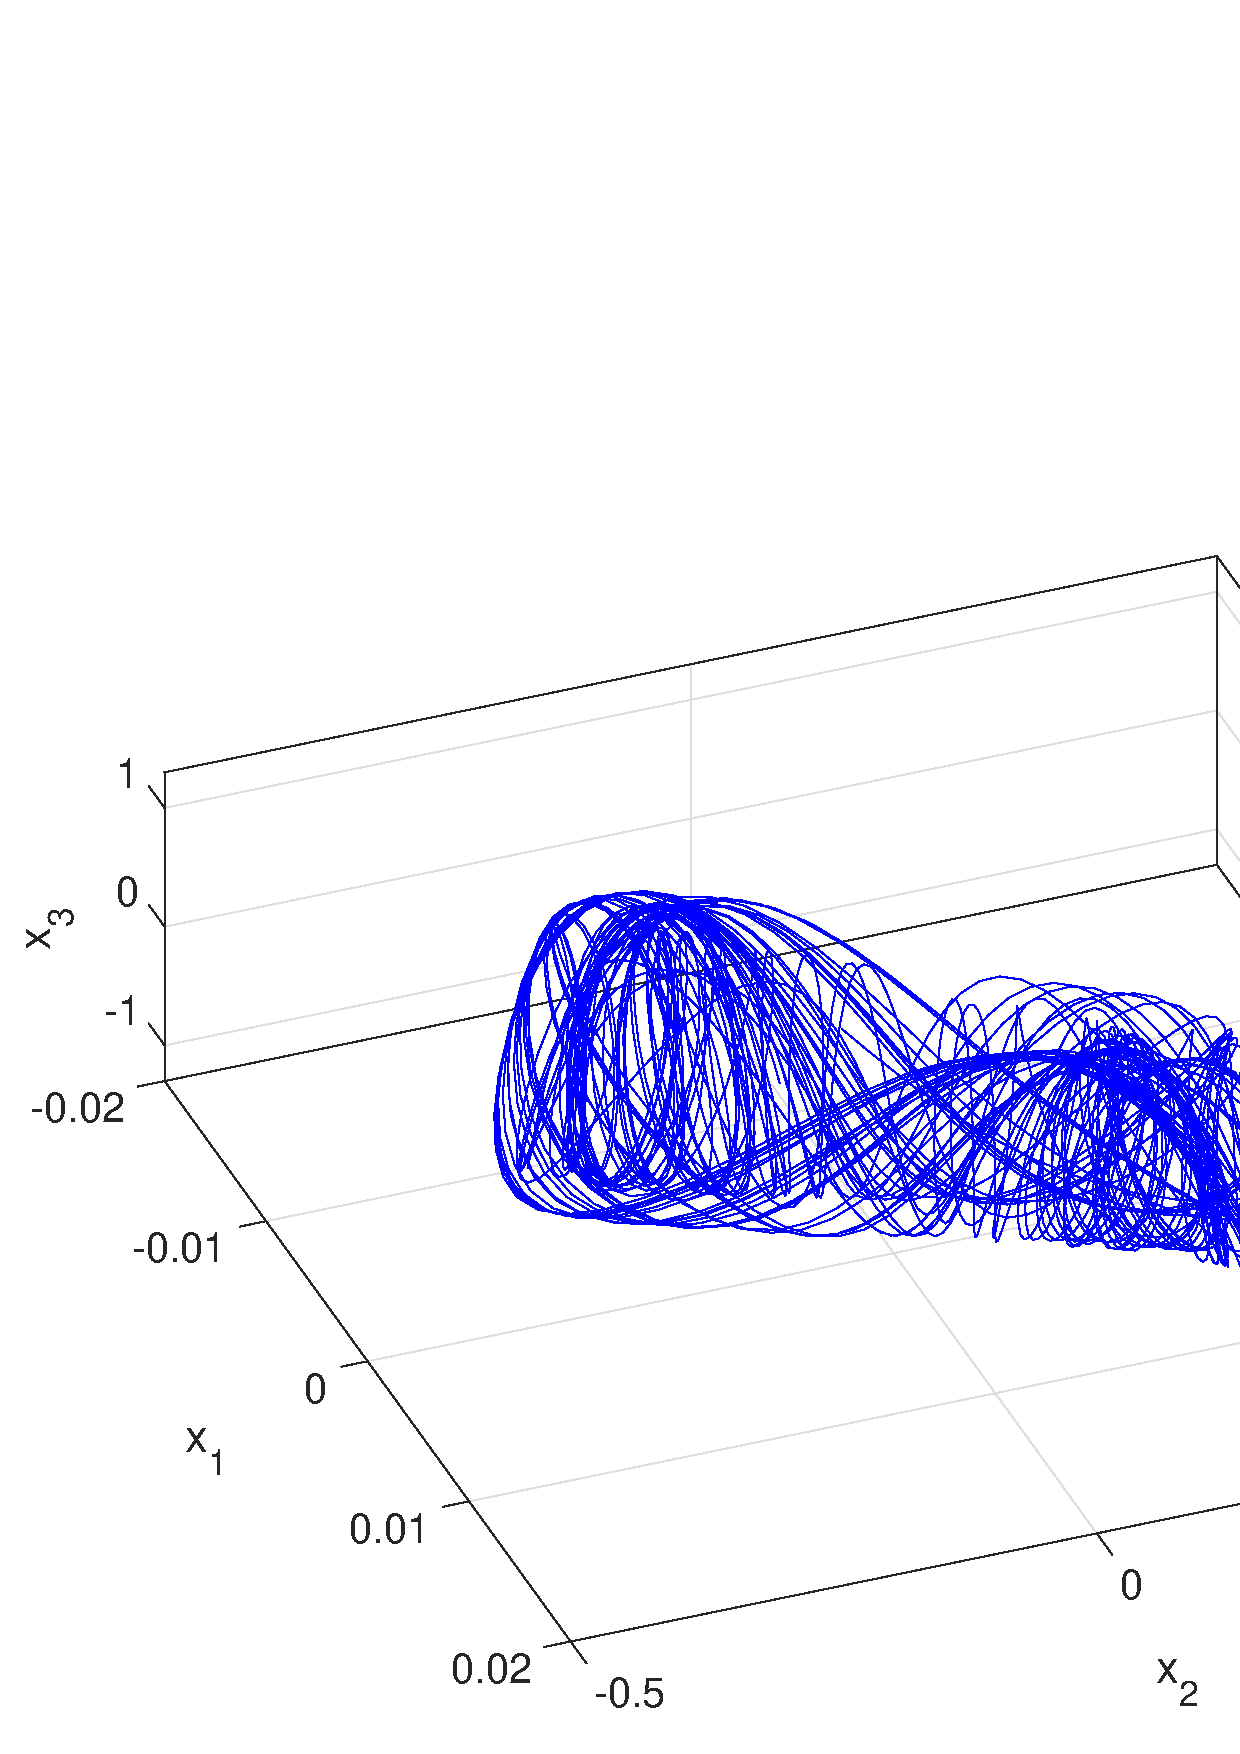
\includegraphics[width=\textwidth]{matcont/StranoAttrattore}
        \caption{Simulazione di un'orbita nello strano attrattore.}
    \end{subfigure}
    \par\bigskip
    \begin{subfigure}{0.85\textwidth}
        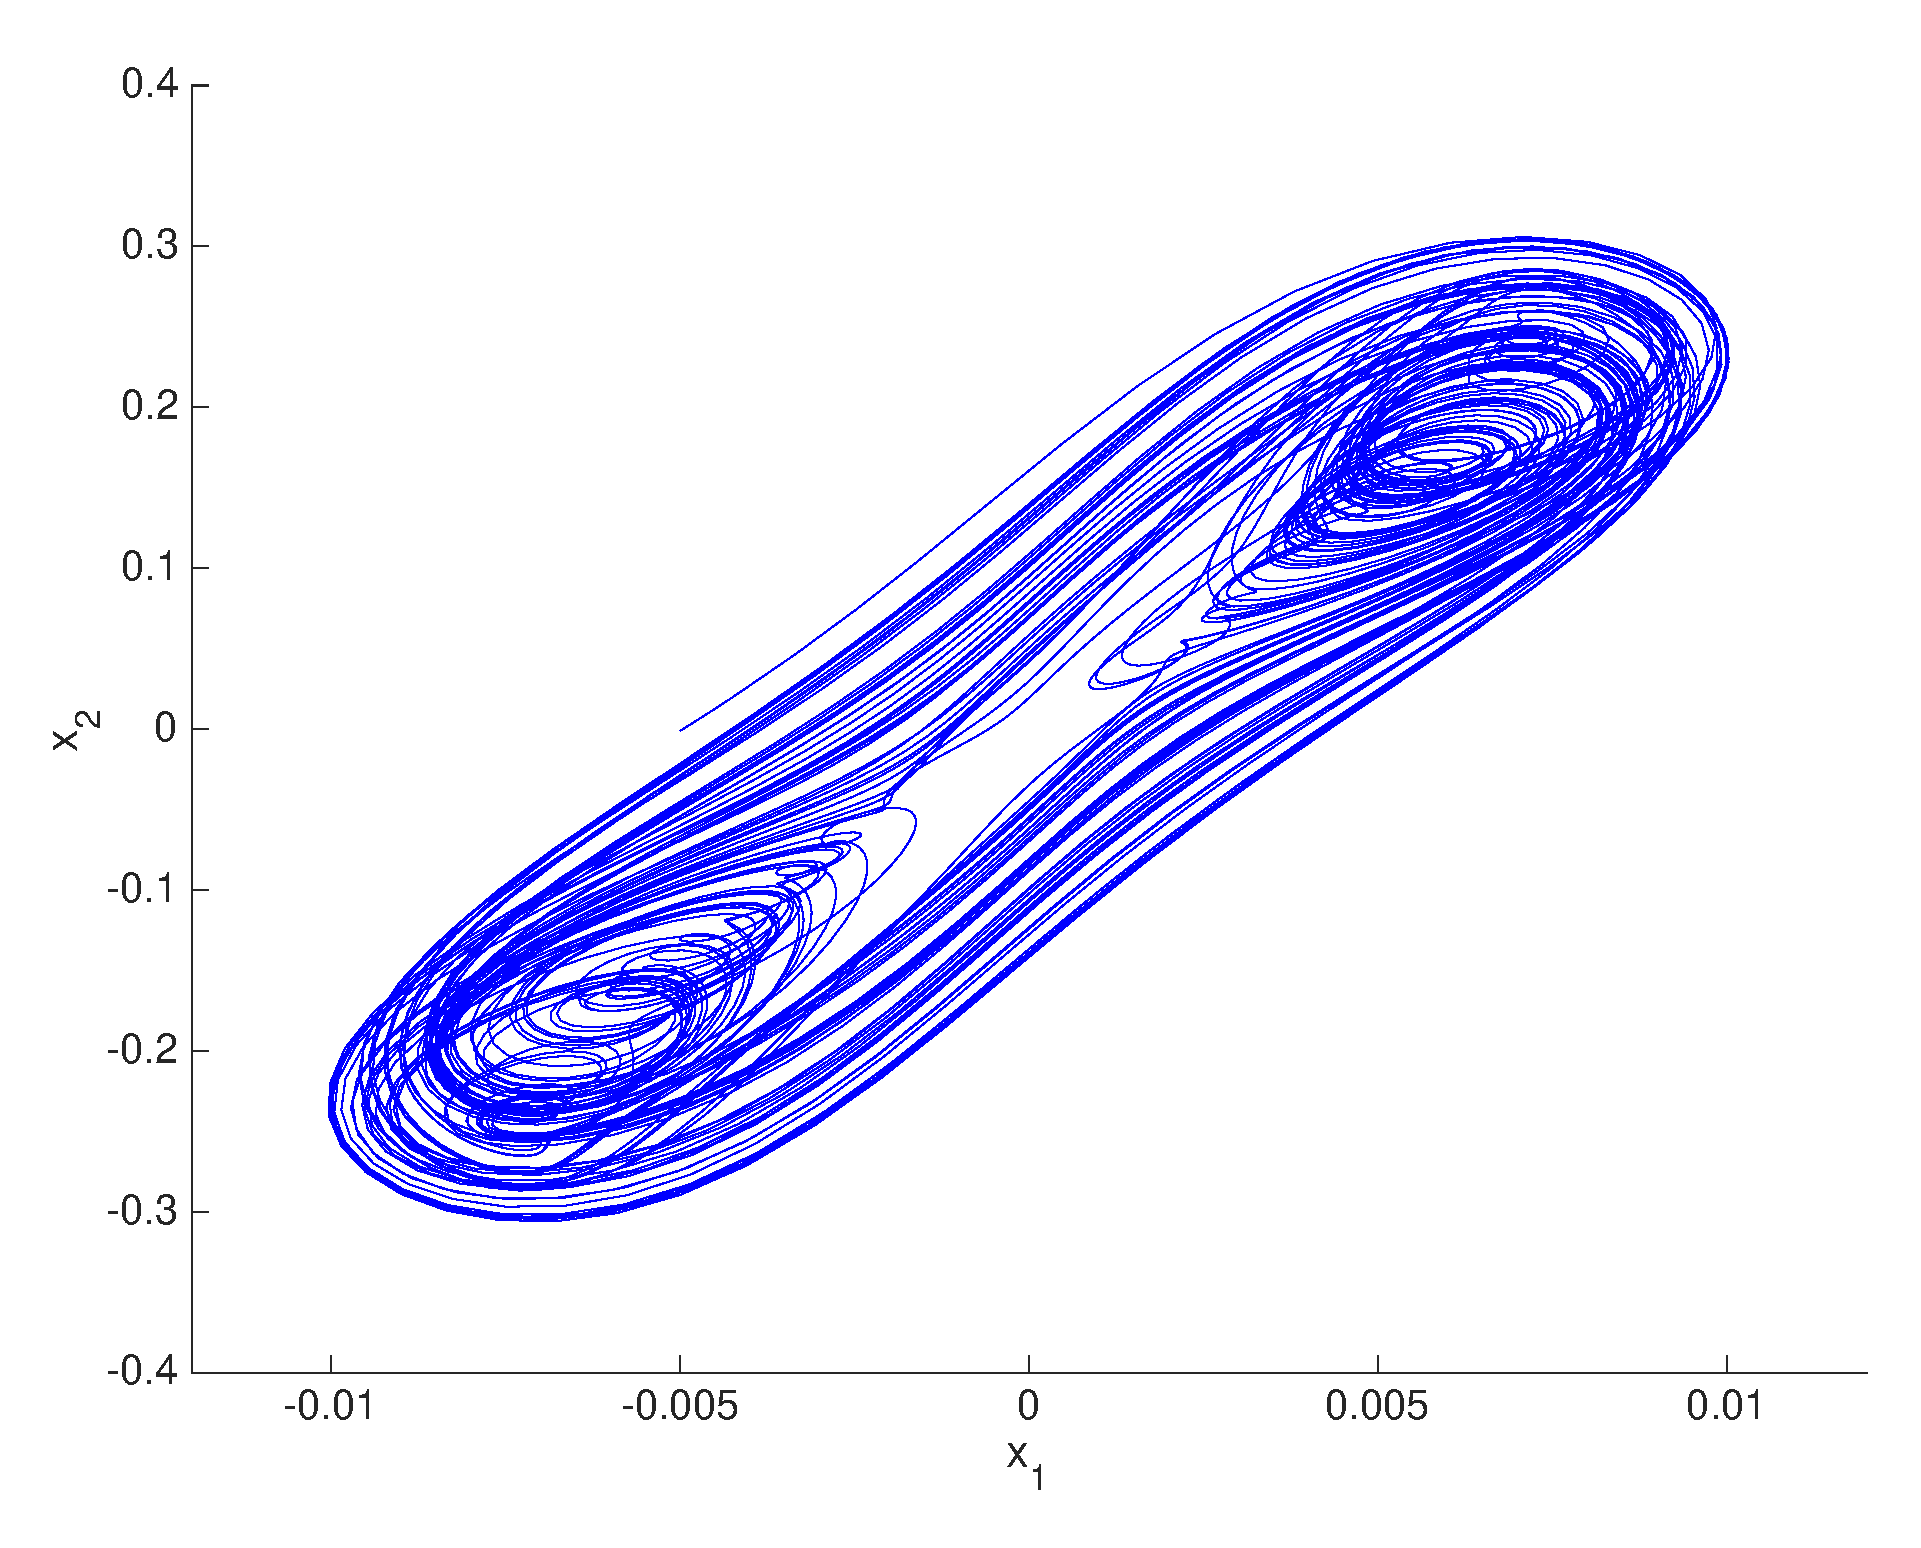
\includegraphics[width=\textwidth]{matcont/StranoAttrattore2D}
        \caption{L'orbita vista ``dall'alto'', sul piano $x_1 x_2$.}
    \end{subfigure}
    \caption{Lo strano attrattore che si ottiene simulando il sistema per $\bar{R}=29.5 \Omega, \omega = 3.1415$.}
    \label{fig:strano-attrattore}
\end{figure}


\end{enumerate}
\end{document}
